\section{问题重述}
\subsection{问题背景}
光伏发电能够为小区提供电力，但发电充足的时段与居民集中用电的时段未必一致。与外部电网相连的微网，可以从外网购电补充供给，也可以利用储能设备把电量留到以后使用。当光伏有剩余或外网电价较低时充电，在供电不足或电价较高时放电，是协调本地发电与用电需求的一种方式。

这种调控同时受到供电可靠性与购电成本的约束。提前多买电可能造成浪费，买得太少又可能在实际运行中产生高价补购；电池虽然能缓冲供需变化，却受到储电容量、充放电功率和能量损耗的限制。因此，微网需要根据决策时已经掌握的信息，协调各时段的购电与储能使用，在满足小区负载的前提下尽可能减少费用。

\begin{figure}[htbp]
  \centering
  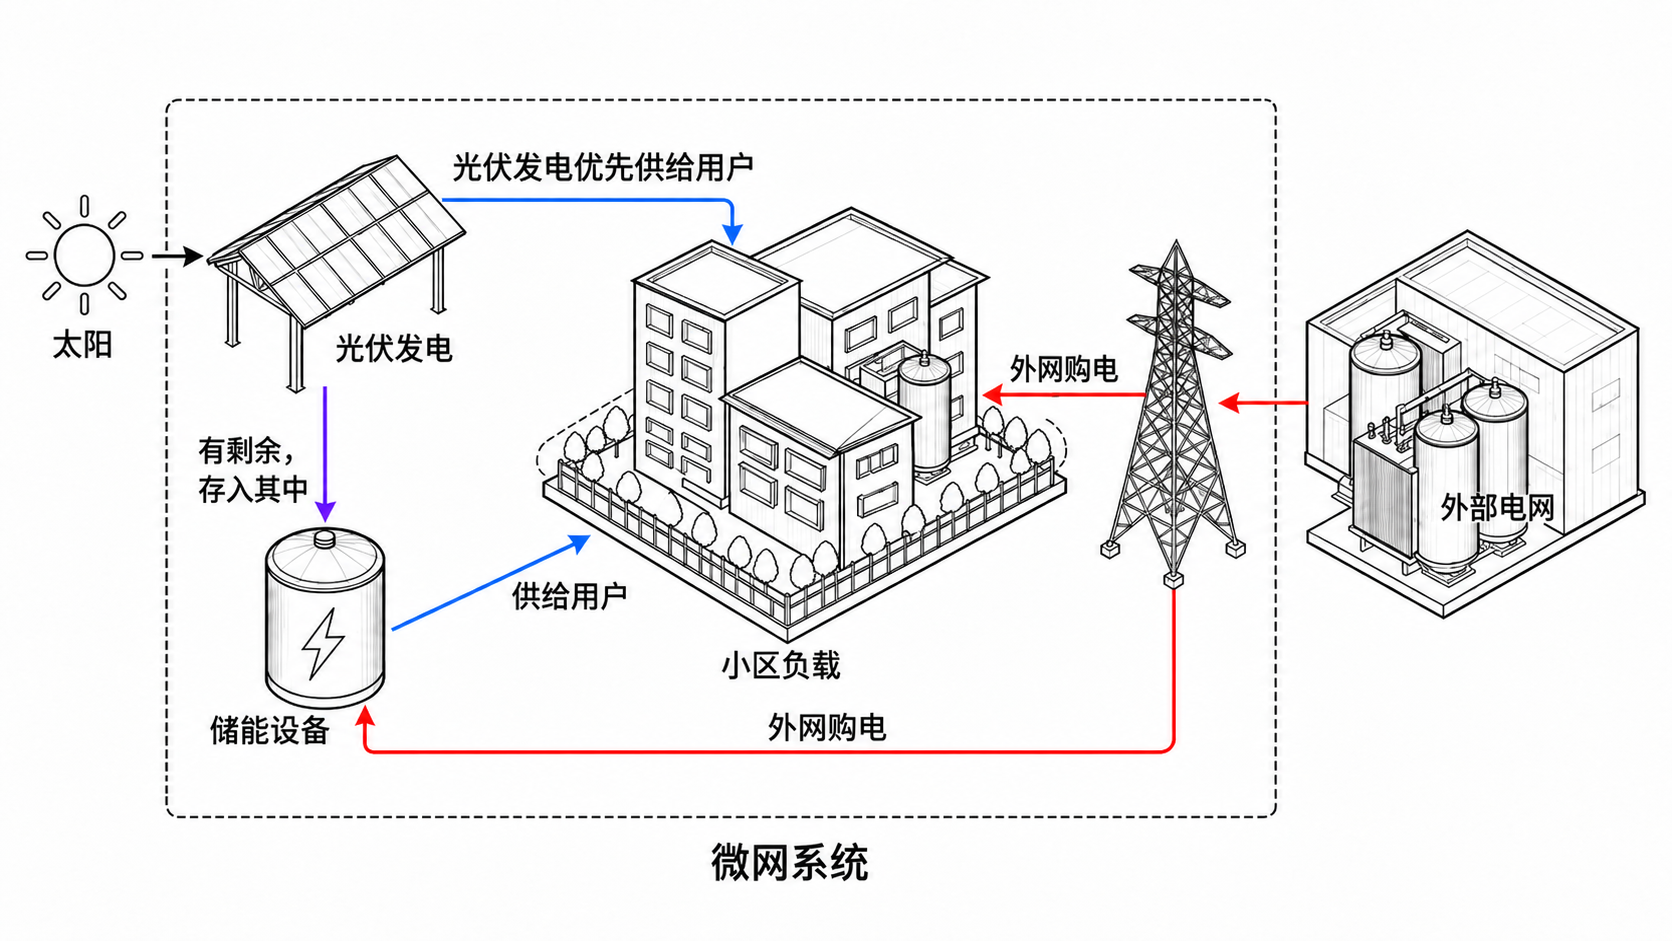
\includegraphics[width=\linewidth,trim=8 8 8 8,clip]{微网系统示意图.png}
  \caption{微网系统的供电关系}
  \label{fig:microgrid-system}
\end{figure}

\subsection{研究对象与共同条件}
研究对象为由光伏、储能设备和外网共同供电的小区微网。附件1给出代表日的电价、负载及光伏预测，附件2给出2025年全年的实际负载和光伏功率，附件3给出每天分四次发布的光伏预报，附件4给出同期波动电价。附件5提供各问的结果文件格式。

储能设备最大容量为12000 kWh，运行储电量须保持在1200--10800 kWh之间，最大充电和放电功率均为5000 kW。题目给定2025年1月1日零点储电量为6000 kWh。功率以kW表示，购电量、充放电量及储电量以kWh表示；各问均须保证微网供电满足小区负载。

\subsection{四问的具体任务}
\textbf{问题一：给定一天供需与电价时的购电安排。}根据附件1和储能参数，在零点安排当天的外网购电及储能充放电，要求当天零点与24点储电量相等。题目中的“每天相同”是指每日重复相同的电价和负载曲线，曲线在一天内仍可随时段变化。需给出满足供电要求、尽可能节省费用的具体安排。

\textbf{问题二：实际供需变化下的每日购电计划。}保持附件1的日内电价，利用附件2所对应的实际运行情景，在每天零点制定当天计划。普通购电按计划量计费；实际运行中供给不足的部分通过紧急购电补足，价格为相应电价的5倍。需同时给出每日计划、实际储能使用及紧急购电情况。

\textbf{问题三：利用更新预报调整购电计划。}在零点取得未来24小时整点光伏预报后制定当天计划，并可在6点、12点和18点取得新预报后调整尚未执行的购电安排。增加的购电量按相应电价的1.5倍收费，减少的部分涉及50\%的违约电价。需给出计划及调整结果，并判断引入日内预报是否值得。

\textbf{问题四：波动电价下的两类购电安排。}使用附件4的电价，分别重新研究问题二和问题三。两条分支分别保留原有的信息条件与调整权限，比较波动电价下的购电、储能使用和费用表现。

\subsection{结果范围与呈现要求}
完整购电结果按10分钟间隔提交。问题一至问题三分别填写\texttt{result1.xlsx}、\texttt{result2.xlsx}和\texttt{result3.xlsx}；问题四的两条分支分别填写\texttt{result4-2.xlsx}和\texttt{result4-3.xlsx}。问题二至问题四的完整结果覆盖2025年2月1日至12月31日，除计划购电和储能记录外，分别保留紧急购电及题目要求的调整记录。

论文按题目指定格式展示重点时段和日期，完整文件保留全部要求的记录。购电展示包括10、12、14、16、18和20点起始的六个10分钟区间，以及全天购电量和费用；储能展示按六个4小时区间分别汇总充电和放电，并列出日初与日末储电量。问题二、三重点展示3月20日、6月21日、9月23日和12月21日，并列出这些日期的紧急购电情况；问题四给出两条分支的相应结果。

\section{问题分析}

\subsection{问题一：已知一天曲线时，电量应当怎样跨时段转移}

问题一给出了完整的日内电价、负载和光伏预测，困难并不在于猜测未来，而在于安排电量何时买、何时存、何时用。光伏最多的时段未必是负载最高的时段，最低电价时段也未必有足够储能空间。若只在低价时尽量充电，电池可能在午间光伏到来前已经装满；若过早放电，又可能在晚间高价和高负载同时出现时失去缓冲能力。因此，需要把全天144个十分钟时段放在一起优化，而不能逐段作出彼此独立的选择。

日初与日末储电量相等是本问的重要条件。它阻止模型通过消耗初始库存制造“今天少买电”的表面低费用，使各方案在相同起点和终点下比较。基于这一结构，问题一采用\textbf{全时段电量流线性规划模型}，将外网直供、外网充电、光伏充电、电池放电和储电量变化统一写入一个优化问题。

\subsection{问题二：计划在零点确定，真实供需随后才出现}

问题二的普通购电必须在每天零点确定，而当天真实负载和光伏还没有发生。附件中的全年数据只能作为事后运行记录和此前历史，不能当作零点已经知道的未来。负载有较明显的星期规律，光伏更受近期天气与季节变化影响，因此二者需要分开预测；预测完成后再合成为净需求，才能保留各自的现实含义。

本问的费用具有明显的不对称性。多订的普通电即使用不完也要付款，少订后真正缺电的部分却要按五倍电价紧急购买。电池能吸收一部分偏差，但会受到最低储电量和放电功率限制，因而“全天总电量够”并不代表每个时段都不会缺电。模型既要给出通常情况下的供需判断，又要依据近期发生过的低估误差留出适量准备。由此采用\textbf{周期预测--近期加权准备--跨日线性规划模型}，并让日末库存自然传给下一天，使当前订电不会把风险简单推迟到次日。

\subsection{问题三：新预报是否值得用，取决于它能否覆盖改单成本}

问题三允许在6:00、12:00和18:00得到新的光伏预报后调整未来订单。新增信息有助于纠正零点判断，但修改订单需要支付调整费，电池也可能已经足以消化预测变化。因此，“获得新预报”和“必须改单”是两件事。合理策略应当先更新未来净需求和实际库存，再比较维持原订单、调增、调减和可能紧急购电的代价。

附件3按小时给出光伏预报，而购电结果按十分钟填写。相邻整点之间采用线性插值，使预报与144个运行时段对应；附件2中的实际光伏只在时段发生后用于更新误差和库存。官方预报反映当天信息，近期同刻历史提供稳定参照，两者各有作用。因而采用\textbf{历史融合预报--动态安全准备--日内滚动规划模型}，并在每个发布时间只调整尚未执行的区间。评价后发预报时，还要把“允许日内反馈和改单”的收益与“新增官方预报”的收益分开，否则会夸大预报本身的贡献。

\subsection{问题四：未来价格也未知后，购电时点本身需要重新判断}

问题四把固定电价改为波动电价。电价变化不只是把原订单重新计价，还会改变什么时候适合充电、什么时候应保留电量以及什么时候放电。因此，需要先用决策时已经发生的价格和历史规律判断未来价格，再把预测价格送入购电与储能规划。

两条分支的权限不同。问题四-2仍在零点一次确定当天普通订单，无法利用当天已发生价格修正，因此更需要表达历史价格、净负荷、星期和季节之间的非线性组合，采用\textbf{滚动提升树--零点线性规划模型}。问题四-3可以在日内更新，价格特征之间相关性较强，又需要解释每次修正来自哪里，因此采用\textbf{滚动岭回归--日内调整线性规划模型}。两种价格模型都只提供决策时的未来判断，最终费用仍按实际电价和真实运行结果结算。


\subsection{四问之间的联系}
四问围绕同一供电系统展开，共享负载满足、光伏利用、储电量变化及设备容量和功率限制。研究首先从问题一的一天安排入手，理清购电与储能转移电量之间的关系；再在问题二中加入实际供需偏差、紧急补购和跨日衔接，使当天计划与实际执行相区分。问题一形成的购电方案仅用于问题二首日启动，后续日期的计划则依据逐日积累的信息制定。

问题三在这一基础上引入按发布时间获得的光伏预报及有代价的计划调整，重点考察提前纠正偏差的作用。问题四分别扩展问题二和问题三，将固定日内电价替换为决策时尚未知晓的波动电价。这样，四问可以共用供电与储能的基本关系，同时分别处理供需偏差、信息更新和价格不确定性；费用比较也可明确对应到普通购电、调整和紧急购电三个来源。
